\begin{figure}[h]\centering
    \pgfplotsset{scaled y ticks=false}
    \begin{tikzpicture}
        \begin{axis}[
            ybar,
            ylabel={kilobytes},
            title={Size of executable},
            width=0.7\textwidth,
            height=0.4\textheight,
            symbolic x coords={GPSW, YCT},
            xtick=data,
            ymin=0, ymax=175,
            bar width=2cm,
            enlarge x limits = 0.75,
            nodes near coords,
            every node near coord/.style={
                /pgf/number format/precision=2
            },
        ]
        \addplot coordinates {
            (GPSW, 148.824)
            (YCT,	88.288)
            % (CCCC, 20000)
        };
        % \addlegendentry{SoC RAM size};
        % \addplot [color=black, mark=none] {262144};
        \end{axis}
    \end{tikzpicture}
    \caption[Flash use of the ABE library executable]{Comparison of the size of the ABE library when using the two schemes.}
    \label{fig:abe-performance-diagrams-flash}
\end{figure}